\chapter{The $s$--$d$-model}\label{ch:sdmodel}
\section{Introduction}
Our model consists of two parts. The first part are the conducting electrons whose Hamiltonian is given by a tight-binding model. These conducting electrons can scatter of impurities in the material leading to having a finite momentum life-time. At the same time the spin of the electrons are coupled to its momentum through spin-orbit interactions, making it possible to transfer this angular momentum to the crystal lattice. The second part is the (anti)ferromagnet which we describe using a Heisenberg model in a classical limit, meaning we replace the spin-operators with vectors. In order to transfer angular momentum between localized and conduction electrons, we therefore need to introduce a parameter that couples the spin and magnetic moment locally. This allows us to directly relate the relaxation of the momentum of conduction electrons to the relaxation of angular momentum of the localized electrons. This momentum relaxation is at the heart of quantum transport theory. This model has much in comparison with the $s$--$d$ model \cite{zener1951interaction,kasuya1956theory,yosida1957magnetic,sdmodel}, used for example in the Kondo effect \cite{10.1143/PTP.32.37}, where localized $d$ electrons are coupled to conduction $s$ electrons through exchange interaction. In the literature therefore our model is often called $s$--$d$, or $s$--$d$-like, and the parameter that couples the spins of localized and itinerant electrons is called an $s$--$d$-like exchange interaction. A related model that is called the $t$--$J$ model is used in the context of high-temperature superconductivity \cite{anderson_resonating_1987, zhang_effective_1988}.

\section{Classical equations of motion on magnetization}\label{cd:sd:motion}
The Hamiltonian describing the localized and conduction electrons is given by
\begin{multline}
    \hat{H}
        = \sum_{\mathclap{\{i,j\}\in\text{n.n.}}}\,\Big(\frac{J_{\text{ex}}}{n}\hat{\bb{S}}_i\cdot\hat{\bb{S}}_j - \frac{K}{2n}\hat{\bb{S}}_{z,i}\cdot\hat{\bb{S}}_{z,j}-t_h \hat{c}_i^\dagger\hat{c}_j
        \Big)\\-\sum_i \big(\mu_s\bb{H}_\text{ext}\cdot\hat{\bb{S}}_i-J_\text{sd}\hat{\bb{S}}_i\cdot\hat{c}_i^\dagger\bb{\sigma}\hat{c}_i\big)+H_\text{tb},
    \label{intro:eq:Hm}%-\lambda i c_i^\dagger \bb{u}_{ij}\cdot\bb{\sigma}\hat{c}_j
\end{multline}
with the Heisenberg exchange energy $J_{\text{ex}}$, anisotropy constant $K$, $s$--$d$-like exchange energy $J_{\text{sd}}$, creation operators for conduction electrons and localized spins $\hat{c}^\dagger_l$ and $\hat{S}$ respectively, Pauli-matrices $\bb{\sigma}$, external magnetic field $\bb{H}_\text{ext}$, magnetic moment of localized electrons $\mu_s$ and a tight-binding Hamiltonian for conducting electrons $H_\text{tb}$.  The first sum is taken over nearest neighbor sites. Note that the constant $K$ is inserted here phenomenologically, but can be computed as done later in Chapter~\ref{ch:baglay} for a honeycomb antiferromagnet.

To describe the full dynamics of the system we assume that the expectation value of of the localized electrons' spins move on a much larger time-scale than the spin-polarization of the conducting electrons. This allows us to decouple the system in two parts. We first derive equations of motion for the localized spins in a classical, mean-field approach by using only the expectation value of conducting electrons spin-polarization. Second, the spin-polarization of the conducting electrons is computed microscopically using linear response theory in response to electric currents and time-derivative of magnetizations, where the localized spins enter as classical fields. 

We can obtain a mean-field form of the Hamiltonian Eq~(\ref{intro:eq:Hm}) by making the replacement
\begin{equation}
    \sum_{\mathclap{\{ij\}\in\text{n.n.}}} \hat{\bb{S}}_i\cdot\hat{\bb{S}}_j\rightarrow n\langle\bb{S}_j\rangle\cdot\sum_i \bb{S}_i
    \label{eq:meanfield}
\end{equation}
with $n \langle \bb{S}_j\rangle$ the effective field produced by the $n$ nearest neighbors felt by $\bb{S}_i$, where $\bb{S}_i$ is the classical expectation value of $\hat{\bb{S}}_i$.  When $J_\text{ex}<0$, the spins favor parallel alignment and the energy can be written as
\begin{equation}
    E = \sum_{i} \Big(\mu_s \hat{\bb{S}}_i\cdot \bb{H}_{\text{ext}}
    - \frac{K}{2}(\hat{S}_{z,i})^2
    -J_{\text{sd}}\mathcal{A}\big(\bb{S}_i\cdot\bb{s}\big)
        \Big)
        \label{intro:eq:E1}
\end{equation}
where we made the replacement
\begin{align}
    \hat{\bb{S}}_i\cdot\hat{c}_i^\dagger\bb{\sigma}\hat{c}_i \rightarrow \bb{S}_i\cdot\bb{s}, \quad \bb{s} = \mathcal{A}^{-1}\langle \hat{c}^\dagger \bb{\sigma}\hat{c}\rangle,
\end{align}
with spin-density polarization $\bb{s}$ and unit cell area $\mathcal{A}$. This replacement follows from the assumption that the dynamics of $\bb{S}$ is much slower than $\bb{s}$. With this assumption we are allowed to take the statistical average of $\hat{c}_i^\dagger\bb{\sigma}\hat{c}_i$, while $\bb{S}_i$ is taken as a constant.

In the case when $J_\text{ex}>0$ the spins favor antiparallel alignment and the energy can be written as
\begin{equation}
    E = \sum_{i} \Big(J_{\text{ex}}\bb{S}^\text{A}_i\cdot\bb{S}^\text{B}_i 
    - \frac{K}{2}((\hat{S}_{z,i}^\text{A})^2+(\hat{S}_{z,i}^\text{B})^2)
    -J_{\text{sd}}\mathcal{A}\big(\bb{S}^\text{A}_i\cdot\bb{s}^\text{A}+\bb{S}^\text{B}_i\cdot\bb{s}^\text{B}\big)
        \Big)
        \label{intro:eq:E2}
\end{equation}
where we introduced the spin polarization density $\bb{s}^\text{A(B)} = \mathcal{A}^{-1}\langle \hat{c}^\dagger \bb{\sigma}\hat{c}\rangle$ (with unit cell area $\mathcal{A}$). 

The equations of motion is given by $\partial_t \bb{S}_i = \{E,\bb{S}_i\}_p$, where $\{\cdots\}_p$ is the Poisson bracket. For angular momenta we simply have $\{\hslash \bb{S}_i,\hslash \bb{S}_j\}_p=\hslash \bb{S}_i\times\bb{S}_j$. As is common practice, the magnetization in the ferromagnet is expressed in terms of a unit vector $\bb{m} = -\bb{S}/|\bb{S}|$ and for an antiferromagnet we introduce the magnetization $\bb{m}$ and staggered magnetization (also called the N\'eel vector) $\bb{n}$ as
\begin{align}
 	\bb{m} & =-1/2(\bb{S}^\text{A}+\bb{S}^\text{B})/|\bb{S}|\\
    \bb{n} & =-1/2(\bb{S}^\text{A}-\bb{S}^\text{B})/|\bb{S}|.
\end{align} 
With these considerations we find the following equations of motion of magnetization for a ferromagnet
\begin{align}
	\hslash \partial_t \bb{m}  & = \bb{m}\times\big(-\mu_s\,\bb{H}_\text{ext}+KS \,\bb{m_z}+\Delta_\text{sd}\,\bb{s}\big)
	\label{intro:eq:S1}
\end{align}
and the following for an antiferromagnet
\begin{align}
\hslash \partial_t \bb{n} = &  -2SJ_\text{ex}\, \bb{n}\!\times\!\bb{m} \nonumber\\
     &  + KS \big(\bb{m}\!\times\!\bb{n}_\perp+\bb{n}\times\bb{m}_\perp\big) 
	+ \Delta_\text{sd} \big(\bb{m}\times\bb{s}^-+\bb{n}\times\bb{s}^+) -\mu_s\bb{n}\times\bb{H}_\text{ext},\\
\hslash \partial_t \bb{m} = & KS  \big(\bb{n}\!\times\!\bb{n}_\perp+\bb{m}\times\bb{m}_\perp\big) 
	+ \Delta_\text{sd} \big(\bb{m}\times\bb{s}^++\bb{n}\times\bb{s}^-)-\mu_s\bb{m}\times\bb{H}_\text{ext}.
	\label{eq:sd:neel}
\end{align}
Here we introduced the notation $\Delta_\text{sd} = J_\text{sd}\mathcal{A}$. In the remainder we will absorb $S$ into $J_\text{ex}$ and $K$ for brevity. 

Note that the mean-field approximation in Eq.~(\ref{eq:meanfield}) is not necessary to obtain Eqs.~(\ref{intro:eq:S1}) \& (\ref{eq:sd:neel}). The same equations of motion can be obtained by first using Heisenberg's equations of motion $i \hslash\partial_t \hat{S}_\alpha = [H,\hat{S}_\alpha]$ (where $\alpha=x,y,z$) and the commutation relations for spin-operators $[\hat{S}_x, \hat{S}_y]=i\hat{S}_z$ on Eq~(\ref{intro:eq:Hm}), and then taking the classical limit $\hat{\bb{S}}\rightarrow \bb{S}$. 

Note that the minus in front of the definitions of $\bb{n}$ and $\bb{m}$ are there because the magnetic moment of electrons are directed in opposite direction of their spin angular moment. Furthermore, although we use the same notation $\bb{m}$ for the magnetization in a ferro and anti-ferromagnet, it is only a unit-vector in the former case and not the latter. 

\section{Spin-torques in ferro- and antiferromagnets}
The dynamics of the magnetization vector in ferromagnets and antiferromagnets are determined by spin-torques. In order to compute a spin-torque, all we need to do is compute the spin-density of the conducting electrons, which is done using linear response theory (see the next section).  
 These torques can be divided into two groups: field-like and damping-like. For antiferromagnets each group can be further subdivided into two: staggered and non-staggered. In a two-dimensional ferromagnet with spin-orbit of Rashba type, the equations of motion are often written phenomenologically as
\begin{equation}
    \partial_t \bb{m} = c_1 \bb{m}\times (\hat{\bb{z}}\times\bb{j}) + c_2 \bb{m}\times\big(\bb{m}\times (\hat{\bb{z}}\times{j})\big) + \alpha \bb{m}\times \partial_t \bb{m},
    \label{eq:sd:ferro}
\end{equation}
where the terms proportional to $c_1$ and $c_2$ are torques that are induced by injecting an electric current $\bb{j}$ and the term proportional to $\alpha$ describes the rate of dissipation of angular momentum and is called Gilbert damping. The field-like and damping-like torques can be identified as those that are respectively even and odd under time-reversal (i.e. changing the signs of $\bb{m}$, $\bb{j}$ and $t$). Note that the spin of the conducting electrons must be odd in time-reversal, so that applying time-reversal on both the magnetic subsystem and the tight-binding model, one will find that the coefficients $c_1$ and $c_3$ are even, while $c_2$ must be odd under total time-reversal. Note that by symmetry we must have that $c_1$ and $\alpha$ are even in scattering time, while $c_2$ is odd in scattering time. In the literature dealing with microscopic theory there is a substantial lack of damping-like torques. The reason is that is it not easy to make $c_2$ odd in scattering time. Since in the current density $\bb{j}$ is already linear in scattering time, one either needs to go beyond linear response or find less trivial mechanisms for the relaxation of angular momentum. For example, we will see in Chapter~\ref{ch:summit} that an damping-like torque appears when the Fermi surface becomes anisotropic. 

Distinguishing between field-like and damping-like torques helps us understand more the dynamics of $\bb{n}$. For example, if the damping-like torques are absent one will only observe a simple precession of the magnetization vector around $\hat{\bb{z}}\times\bb{j}$. Damping-like torques allow for the dissipation of angular momentum so that over time the magnetization vector will be parallel to $\hat{\bb{z}}\times\bb{j}$. The dynamics induced by both field-like and damping-like torques are illustrated in Figure~\ref{fig:llg}. Note that we can change the sign of the damping-like torque by changing the direction of the electric current. If this current-induced damping-like torque overcomes the Gilbert damping one can even reverse the magnetization direction. In such a way one can construct a magnetic memory that stores a "0" or a "1" corresponding to two magnetization directions. This type of switching is illustrated in Figure~\ref{fig:switching_ferro}. The switching rate is determined by the strength of the damping-like torque which is proportional to Rashba spin-orbit coupling and by the strength of magneto-crystalline anisotropy. It is then no surprise that putting a magnetic layer on top of a heavy metal will enhance its magnetic switching abilities. 

In an antiferromagnet we are more interested in the dynamics of the staggered magnetization $\bb{n}$. A phenomenological equation such as Eq.~(\ref{eq:sd:ferro}) can quickly contain ten terms for a antiferromagnet and the dynamics therefore is far more complicated. However, few points can still be made. As can be seen in Eq.~(\ref{eq:sd:neel}), in the absence of conducting electrons and external field, a finite magnetization $\bb{m}$ is enough to induce a precession of $\bb{n}$, typically already in the THz regime (as opposed to the much slower GHz dynamics found in ferromagnets), as the dynamics is driven by the exchange interaction $J_\text{ex}$. In order to produce a switching of the N\'eel vector direction one can use both a field-like torque produced by a staggered spin-polarization and an anti-damping torque produced by a staggered spin-polarization \cite{fjaerbu_electrically_2017, cheng_terahertz_2016, khymyn_antiferromagnetic_2017}.

\begin{figure}
    \centering
    \subcaptionbox{Field-like}{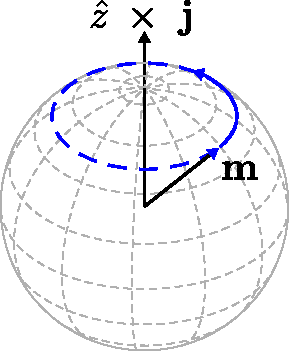
\includegraphics[width=0.31\textwidth]{gfx/llg2}}%
    \hspace{0.2\textwidth}
    \subcaptionbox{Damping-like}{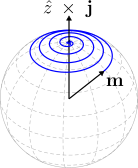
\includegraphics[width=0.31\textwidth]{gfx/llg1}}%
    \caption{Precession of magnetization due to field-like torques (a) and relaxation due to damping-like torques (b). }
    \label{fig:llg}
\end{figure}

\begin{figure}
    \centering
    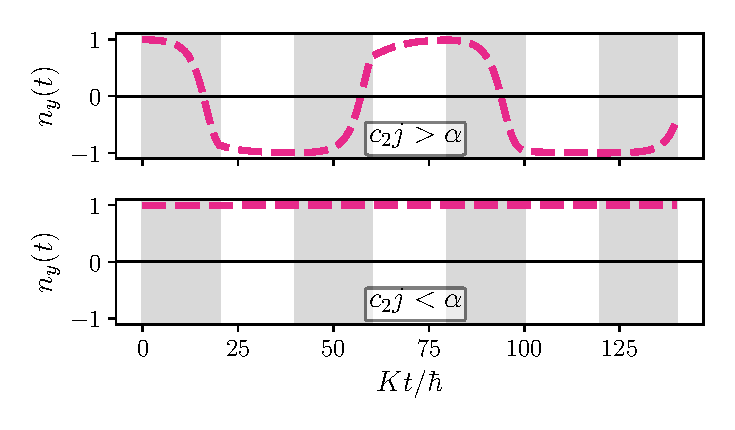
\includegraphics[width=0.95\textwidth]{gfx/switch_ferro}
    \caption{Switching behavior for a Rashba ferromagnet, subject to alternating current pulses. Gray areas correspond to a constant current flowing in the direction of $\pm\hat{x}$, where the sign alternates between each successive box. In the white area the current is switched off. The graph corresponds to numerically solving Eq.~(\ref{eq:sd:ferro}) with values $c_1=0.2$, $j=|\bb{j}|=1$ and $\alpha=0.1$. In the top panel we choose a value of $c_2=0.25$ corresponding to a current overcoming the Gilbert damping making switching possible. In the bottom panel we choose a value of $c_2=0.05$ which corresponds to the opposite case: an insufficiently strong current and therefore no switching. A magneto-crystalline anisotropy term $-K \bb{n}\times\bb{n_y}$ with $K=1$ was included in Eq.~(\ref{eq:sd:ferro}).} 
    \label{fig:switching_ferro}
\end{figure}
\section{Antiferromagnetic resonance}
One of the characteristics of an antiferromagnet is that its antiferromagnetic resonance frequency (i.e. when subjected to an oscillating external magnetic field) is proportional to $\sqrt{K}$, as given by the formula:
\begin{equation}
    \omega = \gamma_0 H_\text{ext} \pm \sqrt{K(J_\text{ex}+K)}
\end{equation}
as first derived by Kittel \cite{PhysRev.82.565, PhysRev.85.329}. The original derivation made use of quadruple contributions to $H_\text{M}$, but for two dimensional systems, a Hamiltonian such as in Eq.~(\ref{intro:eq:Hm}) is sufficient as we will demonstrate. In this section we do not consider $\Delta_\text{sd}$. In order to find the resonant frequencies in the system that is subjected to an oscillating field in the $z$ direction: $\bb{H}_\text{ext} = H_0 \cos \omega t\,\hat{\bb{z}}$, we first linearize the equations of motion by expanding $\bb{n}$ close to $\hat{\bb{z}}$ and assume $\bb{m}$ to be small. To be more explicit
\begin{equation}
	\bb{n} \rightarrow \hat{\bb{z}} + \delta \bb{n}_\parallel,\quad \bb{m} \rightarrow \delta \bb{m}_\parallel.
\end{equation}
Note that to first order the staggered and non-staggered magnetizations are still orthogonal to each-other: $\bb{n}\cdot\bb{m}=1+\mathcal{O}(\delta n^2+\delta m^2)$. Components such as $\delta n_x \delta m_y$ can be then disregarded and we assume $\bb{n}$ and $\bb{m}$ to be proportional to $\exp i \omega t$. A nice basis to work in is $\{{n}_+,{m}_+,{n}_-,{m}_- \}$, (where ${n}_\pm = \delta n_x\pm i \delta n_y$ and ${m}_\pm = \delta m_x\pm i \delta m_y$) so that one finds the following matrix equation:
\begin{equation}
    \begin{pmatrix}
    \omega_0  &  -(J_\text{ex}+K)  &  0  &  0 \\
    -K  &  \omega_0  &  0  &  0 \\
    0  &  0  &  -\omega_0  &  J_\text{ex}+K \\
    0  &  0  &  K  &  -\omega_0
    \end{pmatrix}
    \begin{pmatrix}
    \delta l_{+}\\
    \delta m_{+}\\
    \delta l_{+}\\
    \delta m_{-}
    \end{pmatrix}
    =\omega 
    \begin{pmatrix}
    \delta l_{+}\\
    \delta m_{+}\\
    \delta l_{+}\\
    \delta m_{-}
    \end{pmatrix}
\end{equation}
and four corresponding frequencies $\omega_{\eta',\eta''}$  
\begin{align}
    \omega_{\eta',\eta''} = \eta' \gamma_0 H_\text{ext} +\eta'' \sqrt{K(J_\text{ex}+K)}, \quad \eta',\eta''=\pm1
\end{align}
which remarkably exists even in absence of an external magnetic field. The constant $K$ can be derived directly for a particular model from the Grand potential describing the conducting electrons. The Grand potential is given by
\begin{equation}
    \Omega = - \sum_{\varsigma=\pm}\frac{1}{\beta} \int \mathrm{d}\varepsilon\,g(\varepsilon) \nu_\tau(\varepsilon),
    \label{b1}
\end{equation}
where the the density of states $\nu$ and the function $g(\varepsilon)$ are given by
\begin{align}
    \nu_\tau(\varepsilon) =  &  \frac{1}{\pi} \tr \int \frac{\mathrm{d}^2p}{(2\pi\hslash)^2}\,\im G^\text{R}_{\bb{p}}\\
    g(\varepsilon) =  &  \log \big(1+\exp[\beta(\mu-\varepsilon)]\big).
    \label{eq:nu}
\end{align}
Here $\beta$ is the inverse temperature and $\mu$ is the chemical potential. By evaluating the integral and expanding around the energy minimum in powers of magnetization, one can obtain the anisotropy constant $K$. This will be done explicitly in Chapter~\ref{ch:baglay}.

\section{Obtaining out-of-equilibrium spin-polarizations}\label{diagrammatics}
The spin-polarizations of the conducting electrons that appear in the equations of motion for the ferromagnet Eq.~(\ref{intro:eq:S1}) and for the antiferromagnet Eqs.~(\ref{eq:sd:neel}) are obtained in linear response to current and time-derivatives of magnetizations. This method is used in Chapters~\ref{ch:diffusive},\ref{ch:baglay}, whereas in Chapter \ref{ch:summit} we develop a numerical method of obtaining spin-orbit torques using a scattering approach that will be explained there. 

We can write the linear response of a spin-polarization $s_\alpha$ to a perturbation $H'$ as
\begin{equation}
	s_\alpha = v^2\mathcal{A}\int\!\frac{d^2\bb{p}}{(2\pi)^2}\tr \langle \hat{s}_\alpha G^\text{R}_{\bb{p}} \frac{\partial H'}{\partial t} G^\text{A}_{\bb{p}}\rangle,
\label{sd:eq:kubo2}
\end{equation}
with momentum $\bb{p}$, Fermi-velocity $v$, unit cell area $\mathcal{A}$, retarded (advanced) Green's functions $G^\text{R(A)}_{\bb{p}}$ and operator trace $\tr$. The angular brackets $\langle\dots\rangle$ denote averaging over disorder samples. Eq.~(\ref{sd:eq:kubo2}) is called the Kubo formula that we derive from a Keldysh framework in Appendix~\ref{app:kubo} and is often at the basis of linear response theory. It is in fact one expression of the more general fluctuation-dissipation theorem \cite{Kubo_1966}. This theorem equates the response of a system to an external force or perturbation to the fluctuations of the system in absence of that force or perturbation. In other words, the left hand side of Eq.~(sd:eq:kubo1) denotes an out-of-equilibrium quantity which is related to a correlator on the right hand side that is evaluated in equilibrium. 

The perturbations, or forces, that we consider are (i) electric fields that drive electrons and (ii) changes in magnetization direction. By expressing the electric field in terms of current through the conductivity tensor (which is again obtained through a Kubo formula), we obtain the out-of-equilibrium spin-polarization produced by an electric current. This in turn defines the current-induced spin-orbit torque. The second response, describes how the electrons' spin respond to a change in the electronic spectrum (by varying the magnetization direction) and gives rise to spin-renormalizations and Gilbert damping. 

As mentioned in the introduction of this Chapter we model the relaxation of both spin and orbital angular momentum of conduction electrons through the scattering of impurities. For convenience we choose a white-noise Gaussian disorder potential that is fully characterized by a single dimensionless parameter $\alpha\ll 1$,
\be
\label{disorder}
\la V(\bb{r})\ra =0,\quad \la V(\bb{r}) V(\bb{r}') \ra = 2\pi \alpha\, (\hslash v)^2\,\delta(\bb{r}-\bb{r}'),
\e
where angular brackets stand for the averaging over an ensemble of disordered systems. 

In order to incorporate the effect of disorder, two important steps must be performed. Firstly, we replace the clean Green functions in the linear response formula, with disordered ones. Secondly we replace one of the vertices with one that is corrected with disorder-averaging.

In order to replace the bare Green function with a disordered one, one needs to include a self-energy. This self-energy gives rise to the finite momentum-life-time of the electron and restores translational invariance.  In low concentration of impurities (which we refer to as the clean metal limit, i.e. $\alpha\rightarrow0$) and neglecting contributions from rare-scattering events (such as multiple scattering off the same impurity), one can use the Born approximation

\begin{equation}
\im \Sigma^\text{R(A)} = 2\pi\alpha \im \int \frac{\mathrm{d}\bb{p}}{(2\pi)^2}\,G^\text{R(A)}_{\vec{p},\varepsilon}.
\label{sd:eq:sigma}
\end{equation}

By inserting the self energy into a bare Green function we get the disorder-averaged Green's function
\begin{equation}
	G^\text{R(A)}_{\bb{p}} = \frac{1}{\varepsilon-H_{\bb{p}}-\Sigma^\text{R(A)}}.
\end{equation}
The self-energy determines the poles of the Green's function in the complex energy plane and are equal to the roots of $\det[\varepsilon-H-\Sigma^\text{R(A)}]$. For a given momentum the real part of each pole correspond to a point on a different Fermi surface, while the imaginary part defines the decay of the momentum eigenstates. In other words, the imaginary part gives rise to a finite momentum lifetime. This can be seen by taking the Fourier-transform from energy domain to the time domain where the imaginary part of the pole leads to an exponential decay in time for the Retarded Green's function. To give an explicit example, take for example the Fourier transform with respect to energy of a Green's function belonging to a single particle and single orbital 
\begin{equation}
	G^\text{R}(t) = \int\!\frac{\mathrm{d}\varepsilon}{2\pi} \exp(-i \varepsilon t)\times\underbrace{\frac{1}{\varepsilon-\varepsilon_1+i\varepsilon_2}}_{G^\text{R}(\varepsilon)} = -i\Theta(t)\exp(-i\varepsilon_1t)\exp(-\varepsilon_2 t), 
\end{equation}
where $\Theta$ is the Heaviside step function and $\varepsilon_{1,2}$ are the real and imaginary parts of the the complex energy pole. The temporal Green function decays in time one a time scale set by $\varepsilon_2$. The momentum life-time is defined as $\tau = 1/2\varepsilon_2$ and is equal to the transport time in the Born approximation for isotropic scattering that we consider \cite{rammer_quantum_1986}. The transport-time reflects the time needed to randomize the direction of an electron due to impurity scatterings. Note that in Eq.~(\ref{sd:eq:sigma}) we generally do not explicitly consider the real part of the self-energy as the shift in spectrum can be absorbed into the definition of model parameters. For brevity, we use the same symbols for terms such as Fermi energy and $s$--$d$ energy before and after the Born approximation, but one needs to keep in mind that in the latter case they correspond to renormalized quantities. 

For the second step in disorder averaging, we need to replace one of the vertex functions with one that is corrected for disorder in the ladder approximation (as illustrated in Figure~\ref{sd:fig:diagrams}-b). We call this new vertex function the vertex-corrected function. 
By denoting $\hat{s}^{\text{vc}}$ as the vertex-corrected function of $\hat{s}$ and $\hat{s}^{(i)}$ as the function containing $i$ disorder-lines, the ladder approximation is given by:
\begin{align}
    \hat{s}^\text{vc}
       & =           
        \hat{s}+\hat{s}^{(1)}+\hat{s}^{(2)}+\cdots,
        \label{sd:eq:ladder}
\end{align}
where $\hat{s}^{(i)}$ is given by:
\begin{align}
    \hat{\chi}^\text{i} = 2\pi\alpha_d\int\frac{\mathrm{d}^2\bb{p}}{(2\pi)^2} G_{\bb{p}}^\text{R}\hat{s}^{(i-1)}G_{\bb{p}}^\text{A}
    \label{eq:onedisorderline}
\end{align}

\begin{figure}
    \centering
    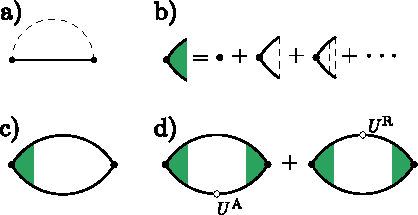
\includegraphics{articles/misha_paper/app5.pdf}
    \caption{Diagrammatic illustration. a) Born-approximation. b) Ladder-approximation. c) Disorder-averaged polarization bubble. d) Perturbative expansion of the disorder-averaged polarization bubble. }
    \label{sd:fig:diagrams}
\end{figure}
This vertex-correction is important as a single scattering event already modifies the spin-polarization. For example we will see in Chapter~\ref{ch:diffusive} that vertex-corrections lead to an unusual and novel torque that we call a diffusive spin-orbit torque. Another example is found in Chapter~\ref{ch:baglay} where disorder averaging can lead to an increase in Gilbert Damping by many orders of magnitude. 

The infinite sum of Eq.~(\ref{sd:eq:ladder}) can actually be recast into a geometrical sum involving matrices. By choosing an appropriate operator basis, $\{\hat{B}_i\}$, where $i=1,2,\dots,n^2$ with $n\times n$ the dimension of the operator space, the vector of vertex corrected basis elements $\bb{B}^\text{vc}\equiv(\hat{B}_1^\text{vc},\dots,\hat{B}_{{n^2}}^\text{vc})$ can written as
\begin{equation}
	\bb{B}^\text{vc} = \bb{B}+\mathcal{F}\bb{B}+\mathcal{F}^2\bb{B}+\mathcal{F}^3+\cdots = \frac{1}{1-\mathcal{F}}\bb{B}.
\end{equation}
By choosing the a basis that satisfies the normalization condition $\tr\bb{B}_i\bb{B}_j=n\delta_{ij}$ we find that the response matrix $\mathcal{F}$ has the following form
\begin{equation}
	\mathcal{F}_{ij} = \frac{2\pi\alpha}{n} \int\!\frac{d^2\bb{p}}{(2\pi)^2}\tr \hat{B}_i G^\text{R}_{\bb{p}} \hat{B}_j G^\text{A}_{\bb{p}}.
\end{equation}
We will see in the remaining chapters that for a Dirac ferromagnet, the operators that we consider only depend on spin-degrees of freedom and therefore the response-matrix has dimension $(2\times2)^2=4\times4$. The Dirac antiferromagnets, however have spin, sublattice and valley degrees of freedom, leading to response-matrices of dimension $(2^3\times2^3)^2=64\times64$. Inverting such a matrix analytically can be a daunting task, but can be simplified dramatically by choosing an appropriate basis and working in certain limits. 

Note that the inversion of $1-\mathcal{F}$ can only be done if none of the eigenvalues of $\mathcal{F}$ is equal to $1$. It appears however that this is never the case, as the self energy expressed in the basis $\{\hat{B}_i\}$ is an eigen function of $\mathcal{F}$ with eigenvalue $1$
\begin{equation}
	2\pi\alpha\int\!\frac{\mathrm{d}\bb{p}}{(2\pi)^2} G^\text{R}_{\bb{p}}\Sigma^\text{R(A)}G^\text{A}_{\bb{p}} = \Sigma^\text{R(A)}.
\end{equation}
In spinless systems we find the same problem in the density-density response which is resolved by working with response functions with finite momentum and frequency. Such a non-local response corresponds to electron diffusion. In Chapter~\ref{ch:diffusive} we will see that for a Dirac ferromagnet this gives rise to a novel type of non-local torque that we call a diffusive spin-torque. In other systems that we studied it appears that the singular eigenvalue in $1-\mathcal{F}$ does not lead to any observable effect. For Rashba ferromagnets it was shown that the divergency appears in the spin-density only in the direction of magnetization. For spin-torque however this plays no role as divergency disappears as the torque is always perpendicular to both the magnetization and spin-density. For the Dirac antiferromagnet that we discuss in Chapter~\ref{ch:baglay} it again appears to play no role on the equations of motion on $\bb{n}$ and $\bb{m}$. It remains an open question what systems, apart from the Dirac ferromagnet, diffusion could play an important role. 
